
\chapter{Software Architecture and Simulation Environments}

This chapter discusses the software architecture of the mobile manipulation robotic system and the simulation 
environments used for testing and development. The software architecture is based on the Robot Operating System 2 (ROS2)
middleware, which provides a flexible and modular framework for developing robotic applications. 
The simulation environments are based on Rviz2 and Ignition Gazebo, which provide realistic simulation environments
for testing the algorithms before deployment on the real robots.

\section{ROS2 Control Interface for Igus Rebel Arm}

The first step in developing the software architecture for the mobile manipulation robotic system is to interface the
Igus Rebel Arm with ROS2. The Igus Rebel Arm is a 6-DOF robotic arm that can be controlled by either the CAN binary bus
or the Ethernet interface (proprietary CRI protocol). The CAN bus interface is used for low-level access to the arm's
joints, while the Ethernet interface is used for high-level control and monitoring of the arm's state. 
The ROS2 control interface for the CAN bus was already implemented by the manufacturer \textit{Commonplace Robotics},
but the requirement was the development of a ROS2 control interface for the Ethernet interface since the CAN bus interface
requires a proprietary cable, which is not available to me. Using the Ethernet interface makes it easier to 
plug it into the switch and control the arm from any computer on the local network.

Developing the \textbf{ROS2 control interface} for the Ethernet interface required understanding the CRI protocol, which
is a protocol based on string messages. The CRI protocol is used to send commands to the arm in the form of
joint positions or velocities (jogs) and to receive feedback from the arm in the form of joint positions.
Controlling the cobot using ROS2 requires a hardware interface, used to command and control the robot by interfacing
with the hardware via the \textbf{CRI protocol}. The hardware interface is implemented as a ROS2 lifecycle node that
is interfaced directly with the Joint Trajectory Controller, which is a ROS2 controller that can be used to
control the arm using joint trajectory messages. This controller is then handled by MoveIt2, which is a ROS2
motion planning framework that can be used to plan and execute trajectories for the arm.

%Add a figure of the control architecture
\begin{figure}[t]
    \centering
    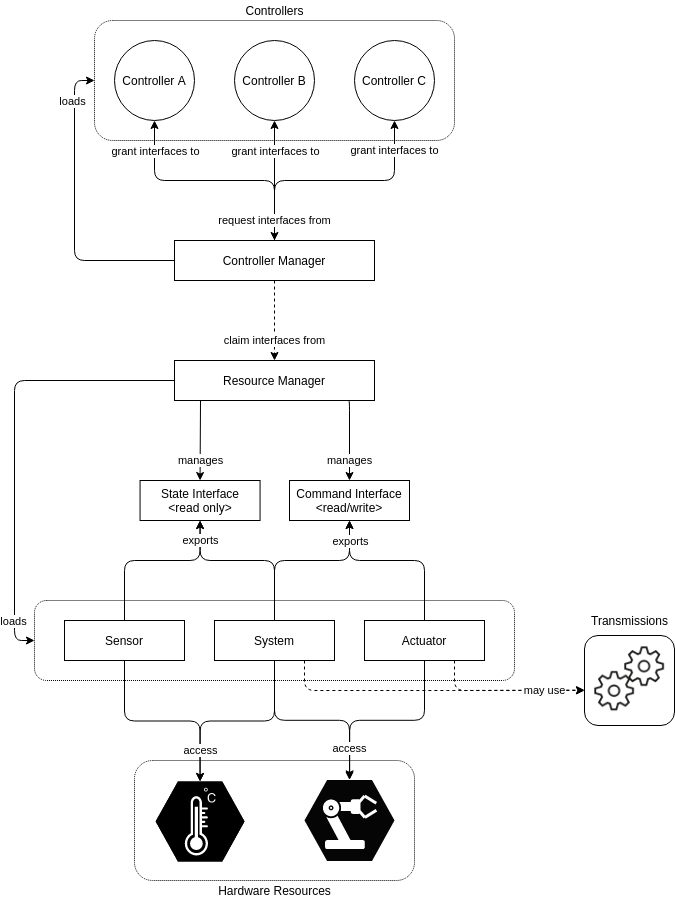
\includegraphics[width=0.6\textwidth]{c4_04.png}
    \caption{ROS2-Control Architecture example}
    \label{fig:ros2control}
\end{figure}

The diagram in figure \ref{fig:ros2control} shows an overview of how \textit{ROS2-Control} works.
The hardware interface implemented for controlling the Igus ReBel arm is a ROS2 lifecycle \textit{System Interface},
which is a type of interface that supports joints and actuators. The system interface accesses the hardware
via the CRI protocol and is managed by the \textit{Controller Manager} and the \textit{Resource Manager}. The
controller manager employed is provided by MoveIt2, in order to handle the cooperation between the hardware
interface and the joint trajectory controller, which receives the computed trajectories from MoveIt2.

\subsection{Joint Trajectory Controller}

The Joint Trajectory Controller is a ROS2 controller that can be used to control the arm using joint trajectory messages.
These messages are joint-space trajectories on a group of joints.
The controller interpolates in time between the points so that their distance can be arbitrary. 
Trajectories are specified as a set of waypoints to be reached at specific time instants, which the controller 
attempts to execute as well as the mechanism allows. Waypoints consist of positions, and optionally velocities and accelerations.

It can be operated either in position, velocity or acceleration mode, depending on the type of trajectory message
that it handles.
The position mode is used to send joint positions to the arm, while the velocity mode is used to send joint velocities
in the form of jog values (velocities in percentage of the maximum velocity). The Joint Trajectory Controller can
be operated either in closed-loop or open-loop mode, depending on the type of feedback that is used to control the arm.
In closed-loop mode, the controller uses the joint positions received from the arm as feedback to adjust the trajectory
to the desired position, by controlling the arm via velocity commands. In open-loop mode, the controller sends the
trajectory to the arm without any feedback, which can be useful for testing the arm's performance without any feedback
control. The closed-loop velocity control requires a PID controller to adjust the velocity commands based on the
difference between the desired and actual joint positions. The PID controller requires tuning of the gains to
achieve the desired performance of the arm. I did not manage to find the best gains for the PID controller,
for a stable and smooth trajectory execution, so I used the open-loop mode for controlling the arm.

MoveIt controller managers, somewhat a misnomer, are the interfaces to your custom low-level controllers. 
A better way to think of them is controller interfaces. The included \textit{MoveItSimpleControllerManager} is sufficient
for the robot controllers that provide ROS2 actions for \textit{FollowJointTrajectory}.

\section{MoveIt2 and RViz2 Simulation Environment}

% Add a figure of the MoveIt2
\begin{figure}[t]
    \centering
    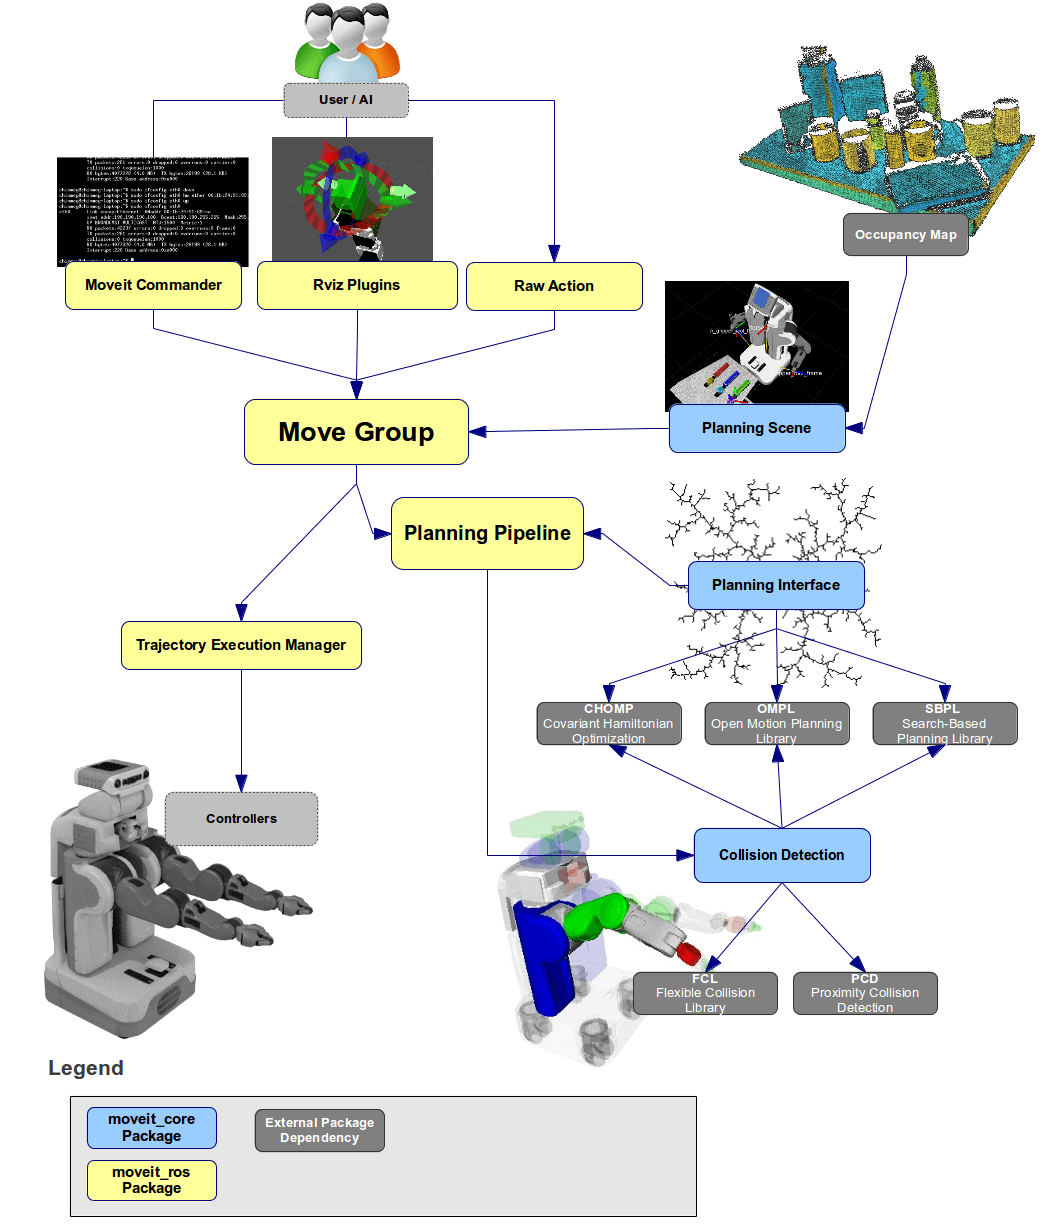
\includegraphics[width=0.8\textwidth]{c4_01.png}
    \caption{MoveIt2 General Architecture}
    \label{fig:moveit2}
\end{figure}

MoveIt2 is a ROS2 framework that provides a set of tools for motion planning, kinematics, control, perception, and
manipulation. It is a powerful tool for controlling robotic arms and mobile bases, and it can be used to plan and
execute trajectories for the arm. MoveIt2 is based on the ROS2 middleware and provides a flexible and modular
framework for developing robotic applications.

The figure \ref{fig:moveit2} shows the general \textbf{architecture of MoveIt2}. The MoveIt2 framework consists of several
components, including the Planning Scene, the Planning Pipeline libraries, the Kinematics Solver, the Collision
Checker, the Trajectory Execution Manager, and the Occupancy Mapping tools.
The Planning Scene is a representation of the robot's environment, including the robot's state, the obstacles in the
environment, and the robot's kinematic model. The Planning Pipeline libraries are used to generate motion plans
for the robot, using the robot's kinematic model and the obstacles in the environment. The Kinematics Solver is
used to compute the robot's joint positions for a given end-effector pose, using the inverse kinematics
computations based on the robot's kinematic model. The Collision Checker is used to check for collisions between
the robot and the obstacles in the environment, using the robot's kinematic model and the obstacles' geometries.
The Trajectory Execution Manager is used to execute the motion plans generated by the Planning Pipeline libraries,
using the robot's joint positions and velocities. The Occupancy Mapping tools are used to generate volumetric 3D 
occupancy maps of the surrounding environment, using depth perception sensors to construct a map
of the obstacles in the environment. 

\begin{figure}[t]
    \centering
    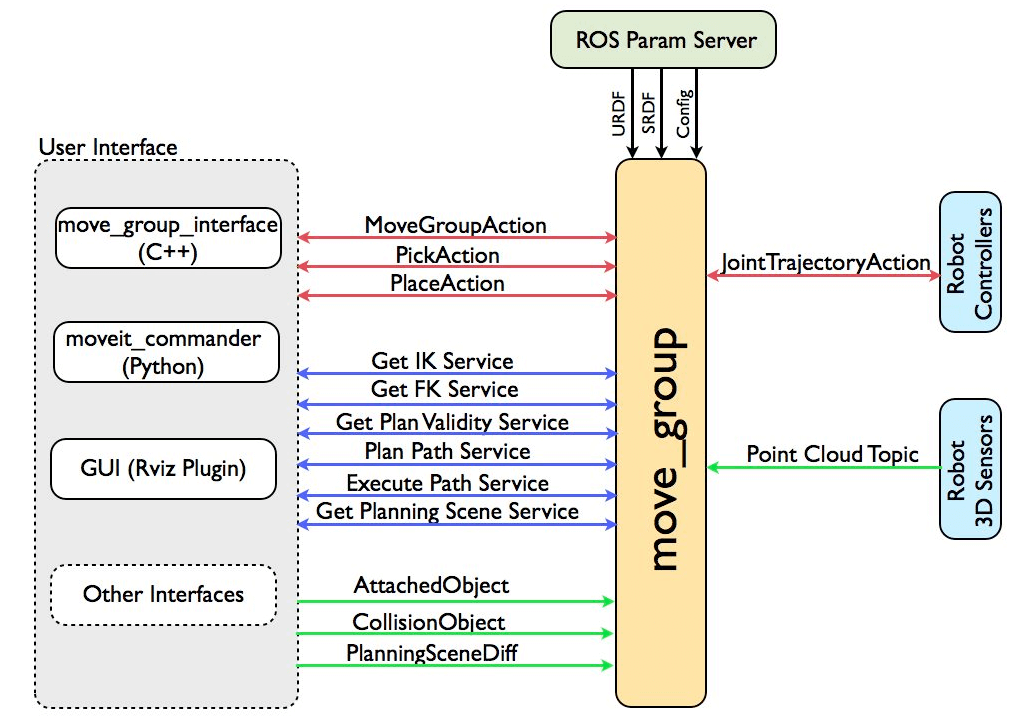
\includegraphics[width=0.8\textwidth]{c4_02.png}
    \caption{MoveGroup Interface}
    \label{fig:move_group}
\end{figure}

MoveIt2 provides the \textit{MoveGroupInterface} class, which is a high-level interface to the MoveGroup class, which is a
class that provides a set of methods for controlling the robot's motion planning and execution. 
Figure \ref{fig:move_group} shows the architecture and the modules with which it interacts.
The \textit{MoveGroupInterface} provides also methods for interacting with the robot's planning scene, 
including adding and removing obstacles, setting the robot's state, and setting the robot's end-effector pose. 
The \textit{MoveGroupInterface} can be used to plan and execute trajectories for the robot. 
It allows to define and compute joint-space goals, Cartesian-space goals,
and pose goals for the robot's end-effector, which is used to compute the joint space trajectories.

%Add a figure of the control architecture
\begin{figure}[t]
    \centering
    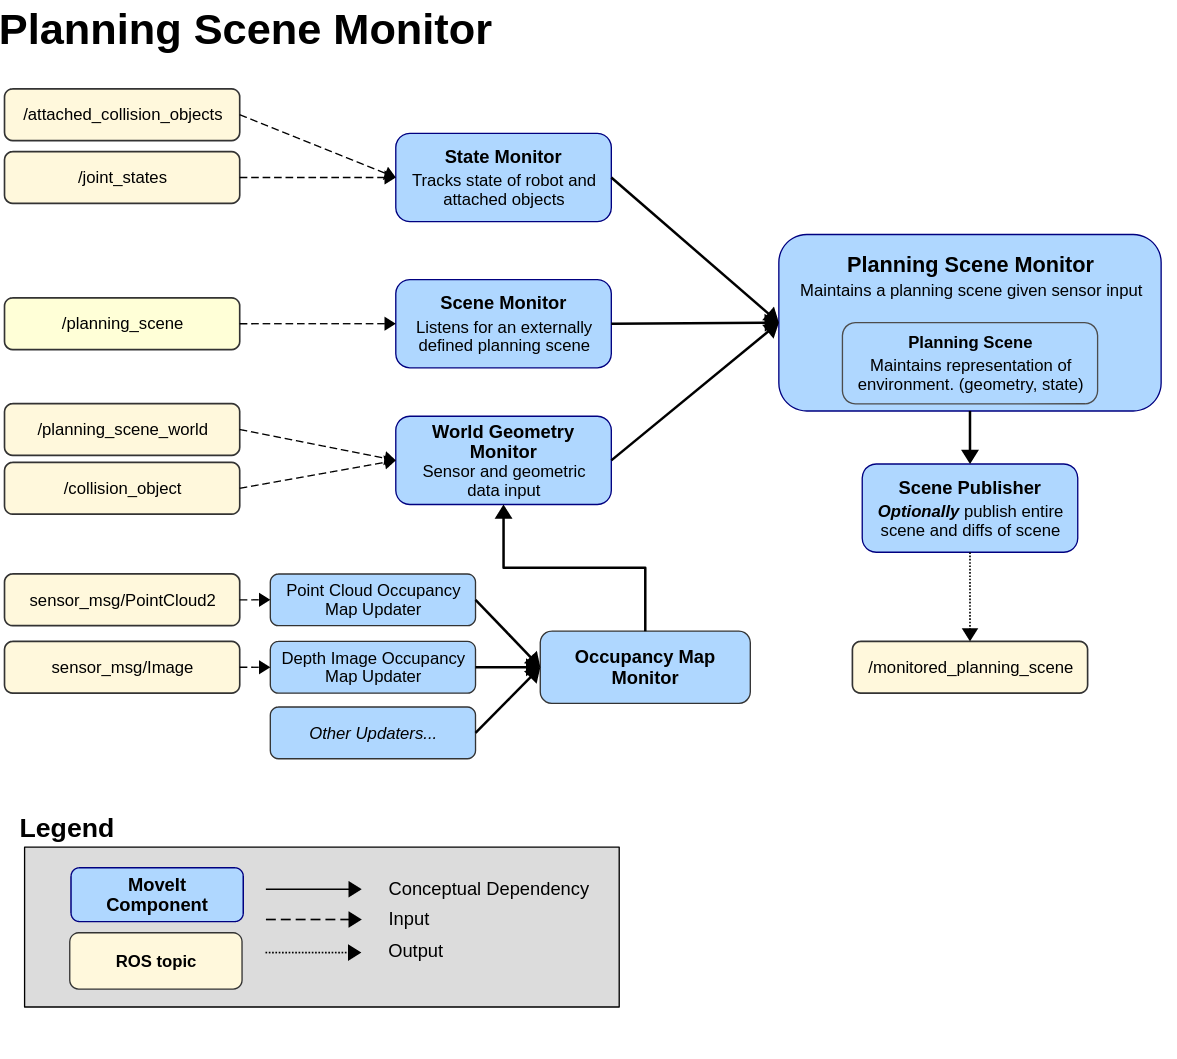
\includegraphics[width=0.8\textwidth]{c4_03.png}
    \caption{Planning Scene and Occupancy Mapping Architecture}
    \label{fig:planninscence}
\end{figure}

MoveIt2 can be used along with RViz2, which is a 3D visualization tool for ROS2 that can be used to visualize the
robot's motion in both simulated and real environments. RViz2 provides a set of tools for visualizing the robot's
kinematic model, the robot's state, the obstacles in the environment, and the robot's motion plans.
Figure \ref{fig:rviz2} shows a screenshot of the RViz2 interface with the control panels dedicated to the MoveIt2
planning and execution tools. With this interface, it is possible to send joint space goals to the robot
and control it via the underlying hardware interface.

%TODO: Add a figure of the rviz2 interface with moveit2
\begin{figure}[t]
    \centering
    %\includegraphics[width=0.8\textwidth]{c4_00.png}
    \caption{RViz2 Interface with MoveIt2 Control Panels and the mobile manipulation robot.}
    \label{fig:rviz2}
\end{figure}

\section{Robotic Arm Visual Servoing}

The MoveIt2 library provides also a framework for visual servo-ing, which is a technique used to control the robot's
end-effector pose using visual feedback from a camera. The visual servo-ing framework in MoveIt2 is based on the
\textit{MoveItServo} package, which provides a set of tools for controlling the robot's end-effector pose using
servo-ing algorithms. The servo-ing algorithms are used to compute the robot's joint positions for a given end-effector
pose. I developed the code to integrate these tools with the camera visual feedback, in order to perform visual servo-ing
experiments with the Igus Rebel Arm. 

The servo-ing algorithms provided by MoveIt2 allow also for \textbf{real-time control and teleoperation} of the robot arm's
end-effector pose. The teleoperation allows the user to control the robot's end-effector pose using a joystick controller.
The real-time control allows the user to control the robot's end-effector pose using camera visual feedback
in real-time without pre-computing the joint trajectories. Realtime control is useful for controlling the robot's
end-effector pose in dynamic environments, where the obstacles are moving and the robot needs to adapt to the changes
in the environment.

\begin{figure}[t]
    \centering
    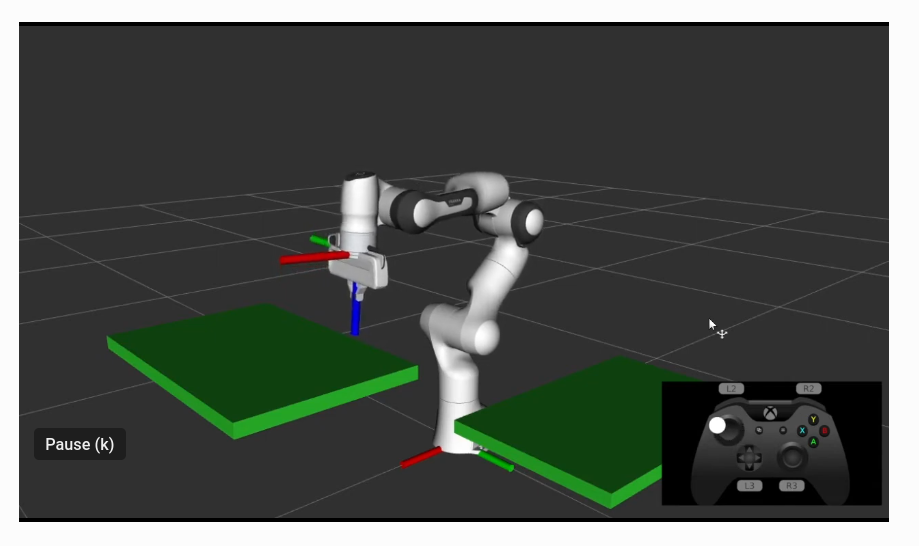
\includegraphics[width=0.8\textwidth]{c4_05.png}
    \caption{Teleoperation with a joystick controller in RViz2 with the Franka Emika Panda}
    \label{fig:teleop}
\end{figure}


After many trials and errors, I managed to get the \textbf{visual servo-ing} working
only with input cartesian poses close to the initial pose of the arm. The servoing algorithm requires
a good initial guess of the end-effector pose, in order to converge to the desired pose.
Since I tested the visual servo-ing with the arm in the open-loop mode, the servo-ing algorithm was not able to
compensate for the errors in the joint positions, which led to the arm not reaching the desired pose.
Then I switched to the closed-loop mode, but the PID controller gains were not tuned properly, which led to strong
oscillations in the joint positions and the arm not reaching the desired pose stably. I did not manage to find the
best gains for the PID controller, so I had to abandon the visual servo-ing experiments with the arm.
The package is still available in the repository, but it is not used in the final implementation
of the mobile manipulation robotic system. Furthermore, the servo-ing algorithms using cartesian input poses
rely exclusively on ROS2-Iron distribution.

\section{Soft Gripper Pneumatic Pump Actuation}

The soft gripper is actuated using a ROS2-control interface that acts as a hardware interface to the Arduino UNO
microcontroller that controls the pneumatic pump. The hardware interface works by providing a ROS2 service server that 
listens for commands to open or close the gripper and sends the corresponding commands to the Arduino UNO microcontroller
via serial communication. The Arduino UNO microcontroller is programmed to control the pneumatic pump by changing
the state of the relays connected to its digital pins. The Arduino UNO listens in the serial port for string commands
that it interprets as the pins to be set high or low, to open or close the gripper. The pneumatic pump is connected
to the Arduino UNO via a relay module with 4 relays, one for each digital pin of the pump. Two of which
are the VCC and GND pins, and the other two are the OPEN and CLOSE pins.


\section{Autonomous Navigation with NAV2}

\subsection{Issues with 3D LIDAR in navigation}

\subsection{Dynamic Obstacle Avoidance with NAV2}

\section{Ignition Gazebo Simulation Environment}

\section{Parking Algorithm for Mobile Robot}

\section{Aruco Marker Detection and Pose Estimation}

\section{Object Detection with YOLOv8}

\section{Collision Avoidance with Octomap}

\section{ROS2 Actions Client-Server Architecture for High-Level Tasks}

